\section{实验要求与实验目的}

\subsection{实验要求}
根据实验指导书，实验二（LED 轮换点亮实验）的要求如下：
\begin{enumerate}
  \item 利用 AT89C51 单片机的 P1 口进行扩展，驱动 LED 灯控制输出。
  \item 编写程序，使 P1.0\textasciitilde{}P1.7 上的发光二极管循环点亮。
  \item 画出 STC89C51/AT89C51 实现上述功能的完整电路图，包括单片机电源、复位电路、晶振电路和控制电路。
  \item 完成全部程序和电路调试工作。
\end{enumerate}

\subsection{实验目的}
\begin{enumerate}
  \item 掌握 AT89C51 单片机并行输出口作为 I/O 输出电路的设计方法。
  \item 学习循环移位指令在流水灯控制中的应用。
\end{enumerate}

\subsection{设计提示}
\begin{enumerate}
  \item 程序设计采用软件延时方法控制灯的轮换速度。
  \item 可采用循环左移指令实现从 P1.0 到 P1.7 的轮换点亮。
\end{enumerate}

\section{Proteus 原理图与硬件电路说明}

\subsection{完整原理图}
\begin{figure}[H]
  \centering
  
\includegraphics[width=0.95\textwidth]{images/ProteusSchematic.PNG}
  \caption{实验二完整原理图}
\end{figure}

\subsection{分电路截图}
\begin{figure}[H]
  \centering
  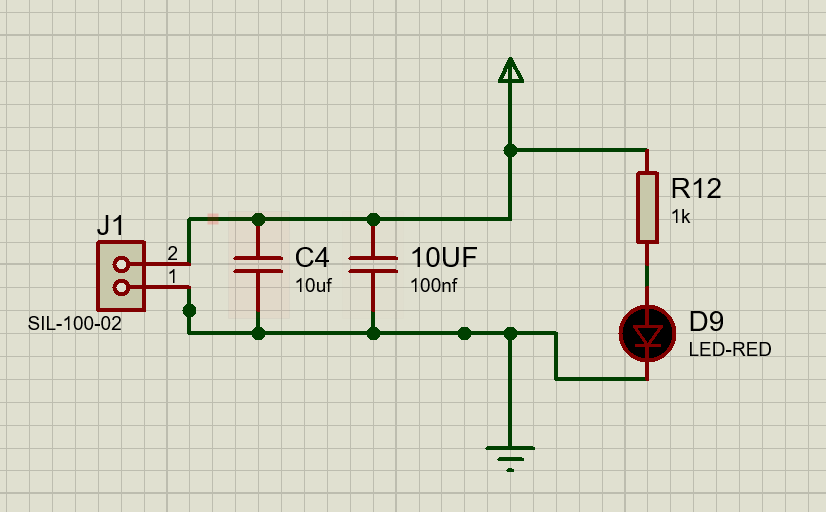
\includegraphics[width=0.72\textwidth]{images/power.PNG}
  \caption{电源电路}
\end{figure}

\begin{figure}[H]
  \centering
  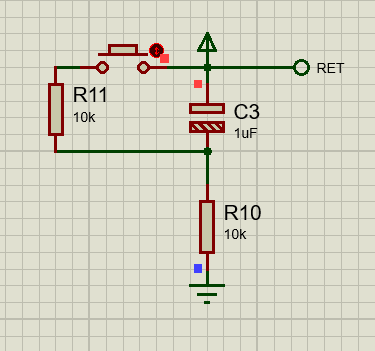
\includegraphics[width=0.55\textwidth]{images/ret.PNG}
  \caption{复位电路}
\end{figure}

\begin{figure}[H]
  \centering
  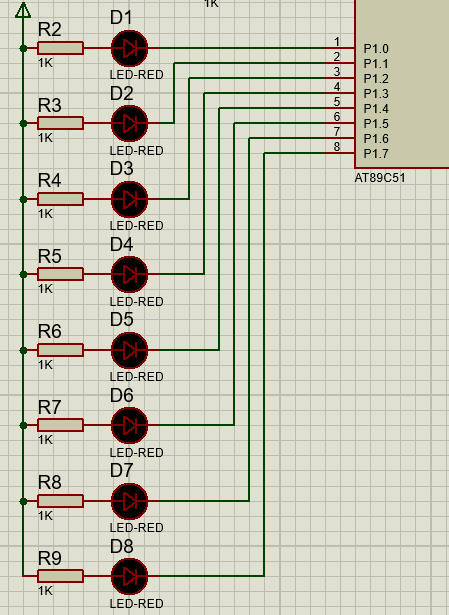
\includegraphics[width=0.58\textwidth]{images/led_control.PNG}
  \caption{LED 控制电路（P1.0\textasciitilde{}P1.7）}
\end{figure}

\subsection{硬件工作原理}
本实验以 AT89C51 为核心，硬件由以下四部分构成：
\begin{itemize}
  \item 电源电路：提供 +5V 稳定供电，并使用电容进行滤波与去耦。
  \item 复位电路：上电后为单片机提供可靠复位脉冲，保证程序从入口地址开始执行。
  \item 晶振电路：由晶振与电容构成时钟网络，提供 MCU 运行时钟。
  \item LED 控制电路：P1.0\textasciitilde{}P1.7 分别连接 D1\textasciitilde{}D8，实现按位输出控制。
\end{itemize}

结合电路连接，程序通过改变 P1 端口输出位模式，实现 8 个 LED 的依次轮换点亮效果。

\subsection{主要元件清单}
\begin{table}[H]
  \centering
  \caption{实验二主要元件与模型}
  \renewcommand{\arraystretch}{1.3}
  \begin{tabular}{cllll}
    \toprule
    序号 & 元件名称 & 元件规格 & 所在元件库 & 所在工具模型 \\
    \midrule
    1 & 单片机 & AT89C51 & Microprcessor & Component mode \\
    2 & 按钮 & BUTTON & Switchs \& Relay & Component mode \\
    3 & 晶振 & CRYSTAL & Miscellaneous & Component mode \\
    4 & 发光二极管 & LED-RED & Optoelectronics & Component mode \\
    5 & 电容 & CAP & Capacitors & Component mode \\
    6 & 电解电容 & CAP-ELEC & Capacitors & Component mode \\
    7 & 电阻 & RES & Resistors & Component mode \\
    9 & 电源 & POWER & Terminals & Terminals mode \\
    10 & 地 & GROUND & Terminals & Terminals mode \\
    11 & 电源输入端 & SIL-100-02 & connectors & Component mode \\
    \bottomrule
  \end{tabular}
\end{table}

\section{软件设计与程序流程}

\subsection{设计思路}
为了实现 LED 轮换点亮，程序采用“单 0 位循环左移 + 软件延时”的方法：
\begin{enumerate}
  \item 将累加器初始化为 \texttt{0FEH}，即仅最低位为 0；
  \item 将累加器值输出到 \texttt{P1}，点亮当前目标 LED；
  \item 调用延时子程序控制切换节奏；
  \item 使用 \texttt{RL A} 循环左移，使“0 位”在 8 位端口中循环移动；
  \item 进入无限循环，得到连续流水灯效果。
\end{enumerate}

\subsection{程序流程图}
\begin{figure}[H]
\centering
\begin{tikzpicture}[
  node distance=10mm and 14mm,
  proc/.style={rectangle,rounded corners,draw=themecolor,fill=blue!3,minimum width=5.2cm,minimum height=9mm,align=center},
  io/.style={trapezium,trapezium left angle=75,trapezium right angle=105,draw=themecolor,fill=cyan!6,minimum width=5.6cm,minimum height=9mm,align=center},
  line/.style={-Latex,thick,draw=themecolor}
]
  \node[proc] (start) {程序开始};
  \node[proc,below=of start] (init) {初始化：\texttt{MOV A, \#0FEH}};
  \node[io,below=of init] (outp) {输出端口：\texttt{MOV P1, A}};
  \node[proc,below=of outp] (delay) {调用延时：\texttt{ACALL DELAY}};
  \node[proc,below=of delay] (shift) {循环左移：\texttt{RL A}};
  \node[proc,below=of shift] (jump) {循环跳转：\texttt{SJMP LOOP}};

  \draw[line] (start) -- (init);
  \draw[line] (init) -- (outp);
  \draw[line] (outp) -- (delay);
  \draw[line] (delay) -- (shift);
  \draw[line] (shift) -- (jump);
  \draw[line] (jump.east) -| ++(1.7,0) |- (outp.east);
\end{tikzpicture}
\caption{LED 轮换点亮程序流程图}
\end{figure}

\subsection{完整实验代码}
\lstset{style=a51style}
\lstinputlisting[caption={02\_flow\_led.A51 完整源码}]{code/02_flow_led.A51}

\subsection{关键代码说明}
\begin{table}[H]
  \centering
  \caption{关键指令与功能说明}
  \renewcommand{\arraystretch}{1.35}
  \begin{tabular}{p{0.30\textwidth}p{0.64\textwidth}}
    \toprule
    指令 & 功能说明 \\
    \midrule
    \texttt{MOV A, \#0FEH} & 初始化输出模式，保证仅一个 LED 处于点亮位。 \\
    \texttt{MOV P1, A} & 将模式输出到 P1 口，驱动 D1\textasciitilde{}D8 中当前目标 LED。 \\
    \texttt{ACALL DELAY} & 调用软件延时子程序，控制视觉上的切换速度。 \\
    \texttt{RL A} & 将累加器按位循环左移，实现点亮位置依次向高位移动。 \\
    \texttt{DJNZ R6, D2 / DJNZ R7, D1} & 双层计数延时，提供稳定时间基准。 \\
    \texttt{SJMP LOOP} & 构成主循环，持续输出流水灯效果。 \\
    \bottomrule
  \end{tabular}
\end{table}

\section{调试过程与实验结果}

\subsection{调试过程记录}
\begin{enumerate}
  \item 根据原理图完成电源、复位、晶振和 LED 控制电路连接。
  \item 加载汇编程序并启动 Proteus 仿真。
  \item 观察 D1\textasciitilde{}D8 是否按顺序轮换点亮。
  \item 调整延时常数，确认轮换速度满足观察要求。
  \item 连续运行，检查是否存在跳灯、乱序或停滞现象。
\end{enumerate}

\subsection{结果验证表}
\begin{table}[H]
  \centering
  \caption{LED 轮换点亮结果记录}
  \renewcommand{\arraystretch}{1.35}
  \begin{tabular}{ccc}
    \toprule
    测试步骤 & 预期现象 & 结果 \\
    \midrule
    1 & D1 点亮，其余熄灭 & 符合 \\
    2 & D2 点亮，其余熄灭 & 符合 \\
    3 & D3 点亮，其余熄灭 & 符合 \\
    4 & D4 点亮，其余熄灭 & 符合 \\
    5 & D5 点亮，其余熄灭 & 符合 \\
    6 & D6 点亮，其余熄灭 & 符合 \\
    7 & D7 点亮，其余熄灭 & 符合 \\
    8 & D8 点亮后回到 D1，循环往复 & 符合 \\
    \bottomrule
  \end{tabular}
\end{table}

\section{问题分析与改进建议}
\begin{enumerate}
  \item 若 LED 切换过快，可增大延时循环计数值提高可视性。
  \item 若出现点亮逻辑相反，应检查 LED 接线极性与端口灌电流方式。
  \item 后续可引入定时器中断替代软件延时，以提高程序可扩展性。
\end{enumerate}

\section{实验结论}
本实验完成了基于 AT89C51 的 LED 轮换点亮控制。程序通过 P1 口并行输出、循环左移指令与软件延时子程序，实现了 D1\textasciitilde{}D8 依次点亮并循环运行。实验验证了并行输出口应用与循环移位指令在单片机控制中的典型用法，达到了实验二要求。
